\documentclass{article}\usepackage[]{graphicx}\usepackage[]{xcolor}
% maxwidth is the original width if it is less than linewidth
% otherwise use linewidth (to make sure the graphics do not exceed the margin)
\makeatletter
\def\maxwidth{ %
  \ifdim\Gin@nat@width>\linewidth
    \linewidth
  \else
    \Gin@nat@width
  \fi
}
\makeatother

\definecolor{fgcolor}{rgb}{0.345, 0.345, 0.345}
\newcommand{\hlnum}[1]{\textcolor[rgb]{0.686,0.059,0.569}{#1}}%
\newcommand{\hlsng}[1]{\textcolor[rgb]{0.192,0.494,0.8}{#1}}%
\newcommand{\hlcom}[1]{\textcolor[rgb]{0.678,0.584,0.686}{\textit{#1}}}%
\newcommand{\hlopt}[1]{\textcolor[rgb]{0,0,0}{#1}}%
\newcommand{\hldef}[1]{\textcolor[rgb]{0.345,0.345,0.345}{#1}}%
\newcommand{\hlkwa}[1]{\textcolor[rgb]{0.161,0.373,0.58}{\textbf{#1}}}%
\newcommand{\hlkwb}[1]{\textcolor[rgb]{0.69,0.353,0.396}{#1}}%
\newcommand{\hlkwc}[1]{\textcolor[rgb]{0.333,0.667,0.333}{#1}}%
\newcommand{\hlkwd}[1]{\textcolor[rgb]{0.737,0.353,0.396}{\textbf{#1}}}%
\let\hlipl\hlkwb

\usepackage{framed}
\makeatletter
\newenvironment{kframe}{%
 \def\at@end@of@kframe{}%
 \ifinner\ifhmode%
  \def\at@end@of@kframe{\end{minipage}}%
  \begin{minipage}{\columnwidth}%
 \fi\fi%
 \def\FrameCommand##1{\hskip\@totalleftmargin \hskip-\fboxsep
 \colorbox{shadecolor}{##1}\hskip-\fboxsep
     % There is no \\@totalrightmargin, so:
     \hskip-\linewidth \hskip-\@totalleftmargin \hskip\columnwidth}%
 \MakeFramed {\advance\hsize-\width
   \@totalleftmargin\z@ \linewidth\hsize
   \@setminipage}}%
 {\par\unskip\endMakeFramed%
 \at@end@of@kframe}
\makeatother

\definecolor{shadecolor}{rgb}{.97, .97, .97}
\definecolor{messagecolor}{rgb}{0, 0, 0}
\definecolor{warningcolor}{rgb}{1, 0, 1}
\definecolor{errorcolor}{rgb}{1, 0, 0}
\newenvironment{knitrout}{}{} % an empty environment to be redefined in TeX

\usepackage{alltt}
\usepackage[margin=1.0in]{geometry} % To set margins
\usepackage{amsmath}  % This allows me to use the align functionality.
                      % If you find yourself trying to replicate
                      % something you found online, ensure you're
                      % loading the necessary packages!
\usepackage{amsfonts} % Math font
\usepackage{fancyvrb}
\usepackage{hyperref} % For including hyperlinks
\usepackage[shortlabels]{enumitem}% For enumerated lists with labels specified
                                  % We had to run tlmgr_install("enumitem") in R
\usepackage{float}    % For telling R where to put a table/figure
\usepackage{natbib}        %For the bibliography
\bibliographystyle{apalike}%For the bibliography
\IfFileExists{upquote.sty}{\usepackage{upquote}}{}
\begin{document}


\cite{Kasdin25} show that dopamine in the brains of young zebra finches acts as 
a learning signal, increasing when they sing closer to their adult song and 
decreasing when they sing further away, effectively guiding their vocal 
development through trial-and-error. This suggests that complex natural 
behaviors, like learning to sing, are shaped by dopamine-driven reinforcement 
learning, similar to how artificial intelligence learns. You can find the 
paper at this link:
\href{https://www.nature.com/articles/s41586-025-08729-1}{{https://www.nature.com/articles/s41586-025-08729-1}.}.

Note they measure dopamine using fibre photometry, changes in the fluorescence
indicate dopamine changes in realtime. Their specific measurement considers 
changes in flourescence in 100-ms windows between 200 and 300 ms from the start 
of singing, averaged across development.

\begin{enumerate}
%%%%%%%%%%%%%%%%%%%%%%%%%%%%%%%%%%%%%%%%%%%%%%%%%%%%%%%%%%%%%%%%%
% CONDUCT A POWER ANALYSIS
%%%%%%%%%%%%%%%%%%%%%%%%%%%%%%%%%%%%%%%%%%%%%%%%%%%%%%%%%%%%%%%%%
\item Using the \texttt{pwr} package for \texttt{R} \citep{pwr},
conduct a power analysis. How many observations would the researchers 
need to detect a moderate-to-large effect ($d=0.65$) when using 
$\alpha=0.05$ and default power (0.80) for a two-sided one sample 
$t$ test.

\begin{knitrout}\scriptsize
\definecolor{shadecolor}{rgb}{0.969, 0.969, 0.969}\color{fgcolor}\begin{kframe}
\begin{alltt}
\hlcom{#Power analysis}
\hlkwd{pwr.t.test}\hldef{(}\hlkwc{d}\hldef{=}\hlnum{0.65}\hldef{,}
           \hlkwc{sig.level}\hldef{=}\hlnum{0.05}\hldef{,}
           \hlkwc{type}\hldef{=}\hlsng{"one.sample"}\hldef{,}
           \hlkwc{alternative} \hldef{=} \hlsng{"two.sided"}\hldef{,}
           \hlkwc{power}\hldef{=}\hlnum{0.8}\hldef{)}
\end{alltt}
\begin{verbatim}
## 
##      One-sample t test power calculation 
## 
##               n = 20.58039
##               d = 0.65
##       sig.level = 0.05
##           power = 0.8
##     alternative = two.sided
\end{verbatim}
\begin{alltt}
\hlcom{#n=20.58 - need at least 21 observations}
\end{alltt}
\end{kframe}
\end{knitrout}
 

%%%%%%%%%%%%%%%%%%%%%%%%%%%%%%%%%%%%%%%%%%%%%%%%%%%%%%%%%%%%%%%%%
% COLLECT DATA
%%%%%%%%%%%%%%%%%%%%%%%%%%%%%%%%%%%%%%%%%%%%%%%%%%%%%%%%%%%%%%%%%
\item Click the link to go to the paper. Find the source data for 
Figure 2. Download the Excel file. Describe what you needed to
do to collect the data for Figure 2(g). Note that you only need the 
\texttt{closer\_vals} and \texttt{further\_vals}. Ensure to 
\texttt{mutate()} the data to get a difference 
(e.g., \texttt{closer\_vals - further\_vals}).

\begin{knitrout}\scriptsize
\definecolor{shadecolor}{rgb}{0.969, 0.969, 0.969}\color{fgcolor}\begin{kframe}
\begin{alltt}
\hlcom{#Pulling data from figure 2}
\hldef{fig2_further} \hlkwb{=} \hlkwd{read_csv}\hldef{(}\hlsng{"further_data.csv"}\hldef{,} \hlkwc{col_names} \hldef{=} \hlsng{"Further"}\hldef{)}
\end{alltt}


{\ttfamily\noindent\itshape\color{messagecolor}{\#\# Rows: 25 Columns: 1\\\#\# -- Column specification --------------------------------------------------------\\\#\# Delimiter: "{},"{}\\\#\# dbl (1): Further\\\#\# \\\#\# i Use `spec()` to retrieve the full column specification for this data.\\\#\# i Specify the column types or set `show\_col\_types = FALSE` to quiet this message.}}\begin{alltt}
\hldef{fig2_closer} \hlkwb{=} \hlkwd{read_csv}\hldef{(}\hlsng{"closer_data.csv"}\hldef{,} \hlkwc{col_names} \hldef{=} \hlsng{"Closer"}\hldef{)}
\end{alltt}


{\ttfamily\noindent\itshape\color{messagecolor}{\#\# Rows: 25 Columns: 1\\\#\# -- Column specification --------------------------------------------------------\\\#\# Delimiter: "{},"{}\\\#\# dbl (1): Closer\\\#\# \\\#\# i Use `spec()` to retrieve the full column specification for this data.\\\#\# i Specify the column types or set `show\_col\_types = FALSE` to quiet this message.}}\begin{alltt}
\hlcom{#Combining 2 values into a single tibble}
\hldef{fig2_tibble} \hlkwb{=} \hlkwd{bind_cols}\hldef{(fig2_further, fig2_closer)}

\hlcom{#Mutating a new column to show the difference between columns}
\hldef{fig2_tibble} \hlkwb{=} \hldef{fig2_tibble |>}
  \hlkwd{mutate}\hldef{(}\hlkwc{Difference} \hldef{= Closer}\hlopt{-}\hldef{Further)}
\end{alltt}
\end{kframe}
\end{knitrout}
To collect the data, I had to first download the source data from the research paper. I could then save the desired variables as .csv files (further and closer), before combining them all into a single tibble. Generating the difference between further and closer just required using \texttt{mutate()}. With these variables, it would be possible to generate Figure 2(g) - the closer values would be on the left, further values on the right, and the difference would represent the lines between them.


%%%%%%%%%%%%%%%%%%%%%%%%%%%%%%%%%%%%%%%%%%%%%%%%%%%%%%%%%%%%%%%%%
% SUMMARIZE DATA
%%%%%%%%%%%%%%%%%%%%%%%%%%%%%%%%%%%%%%%%%%%%%%%%%%%%%%%%%%%%%%%%%
\item Summarize the data.
\begin{enumerate}
  \item Summarize the further data. Do the data suggest that
   dopamine in the brains of young zebra finches decreases when
   they sing further away?
   
\begin{knitrout}\scriptsize
\definecolor{shadecolor}{rgb}{0.969, 0.969, 0.969}\color{fgcolor}\begin{kframe}
\begin{alltt}
\hlkwd{ggplot}\hldef{()} \hlopt{+}
  \hlkwd{geom_histogram}\hldef{(}\hlkwd{aes}\hldef{(fig2_tibble}\hlopt{$}\hldef{Further,} \hlkwc{y}\hldef{=}\hlkwd{after_stat}\hldef{(density)))} \hlopt{+}
  \hlkwd{theme_bw}\hldef{()} \hlopt{+}
  \hlkwd{geom_hline}\hldef{(}\hlkwc{yintercept}\hldef{=}\hlnum{0}\hldef{)} \hlopt{+}
  \hlkwd{xlab}\hldef{(}\hlsng{"Dopamine Compared to Baseline"}\hldef{)} \hlopt{+}
  \hlkwd{ylab}\hldef{(}\hlsng{"Density"}\hldef{)}
\end{alltt}
\end{kframe}
\end{knitrout}

\begin{figre}[H]
\begin{center}
\begin{knitrout}
\definecolor{shadecolor}{rgb}{0.969, 0.969, 0.969}\color{fgcolor}\begin{kframe}


{\ttfamily\noindent\itshape\color{messagecolor}{\#\# `stat\_bin()` using `bins = 30`. Pick better value with `binwidth`.}}\end{kframe}
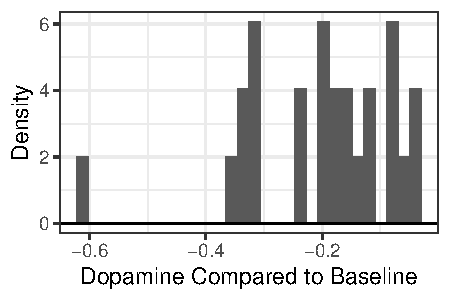
\includegraphics[width=\maxwidth]{figure/unnamed-chunk-4-1} 
\end{knitrout}
\caption{A histogram of birds singing further from adult song}
\label{plot1}
\end{center
\end{figure}




   \item Summarize the closer data. Do the data suggest that
   dopamine in the brains of young zebra finches increases when
   they sing closer to their adult song?
  \item Summarize the paired differences. Do the data suggest
  that there is a difference between dopamine in the brains of
  young zebra finches when they sing further away compared to 
  closer to their adult song?
  \item \textbf{Optional Challenge:} Can you reproduce Figure 2(g)?
  Note that the you can use \texttt{geom\_errorbar()} to plot
  the range created by adding the mean $\pm$ one standard deviation.
\end{enumerate}
%%%%%%%%%%%%%%%%%%%%%%%%%%%%%%%%%%%%%%%%%%%%%%%%%%%%%%%%%%%%%%%%%
% CONDUCT THE TESTS
%%%%%%%%%%%%%%%%%%%%%%%%%%%%%%%%%%%%%%%%%%%%%%%%%%%%%%%%%%%%%%%%%
\item Conduct the inferences they do in the paper. Make sure to report the results
a little more comprehensively -- that is your parenthetical should look something
like: ($t=23.99$, $p<0.0001$; $g=1.34$; 95\% CI: 4.43, 4.60).\\
\textbf{Note:} Your numbers may vary slightly as they performed some unclear
correction of their $p$-values. I'm waiting to hear back from them via email!
\begin{enumerate}
  \item ``The close responses differed significantly from 0 ($p=1.63 \times 10^{-8}$).''

\begin{knitrout}\scriptsize
\definecolor{shadecolor}{rgb}{0.969, 0.969, 0.969}\color{fgcolor}\begin{kframe}
\begin{alltt}
\hldef{mu0} \hlkwb{<-} \hlnum{0}
\hlcom{#Calculating for closer (right-sided)}
\hlcom{#Manually calculating statistics}
\hldef{x} \hlkwb{<-} \hldef{fig2_tibble}\hlopt{$}\hldef{Closer}
\hldef{xbar} \hlkwb{<-} \hlkwd{mean}\hldef{(x)}
\hldef{s} \hlkwb{<-} \hlkwd{sd}\hldef{(x)}
\hldef{n} \hlkwb{<-} \hlkwd{length}\hldef{(x)}
\hldef{t.stat} \hlkwb{<-} \hldef{(xbar} \hlopt{-} \hldef{mu0)}\hlopt{/}\hldef{(s}\hlopt{/}\hlkwd{sqrt}\hldef{(n))}
\hldef{p.val} \hlkwb{<-} \hlkwd{pt}\hldef{(}\hlkwc{q}\hldef{=}\hlopt{-}\hlkwd{abs}\hldef{(t.stat),} \hlkwc{df} \hldef{= n}\hlopt{-}\hlnum{1}\hldef{)}

\hlcom{#Calculating hedges value}
\hldef{closer_hedges_vals} \hlkwb{=} \hlkwd{hedges_g}\hldef{(}\hlkwc{x} \hldef{= x,} \hlkwc{mu} \hldef{= mu0,} \hlkwc{alternative} \hldef{=} \hlsng{"greater"}\hldef{)}

\hlcom{#having t.test calculate values automatically and ensuring they match}
\hldef{closer_t_test} \hlkwb{=} \hlkwd{t.test}\hldef{(}\hlkwc{x}\hldef{=x,} \hlkwc{mu} \hldef{= mu0,} \hlkwc{alternative} \hldef{=} \hlsng{"greater"}\hldef{)}
\hldef{closer_CI} \hlkwb{=} \hlkwd{t.test}\hldef{(}\hlkwc{x}\hldef{=x)}\hlopt{$}\hldef{conf.int} \hlcom{#Caluclating the CI using a two sided test}
\end{alltt}
\end{kframe}
\end{knitrout}
  
  \item ``The far responses differed significantly from 0 ($p=5.17 \times 10^{-8}$).''
  
\begin{knitrout}\scriptsize
\definecolor{shadecolor}{rgb}{0.969, 0.969, 0.969}\color{fgcolor}\begin{kframe}
\begin{alltt}
\hlcom{#Calculating for further (left sided)}
\hlcom{#Manually calculating statistics}
\hldef{x} \hlkwb{<-} \hldef{fig2_tibble}\hlopt{$}\hldef{Further}
\hldef{xbar} \hlkwb{<-} \hlkwd{mean}\hldef{(x)}
\hldef{s} \hlkwb{<-} \hlkwd{sd}\hldef{(x)}
\hldef{n} \hlkwb{<-} \hlkwd{length}\hldef{(x)}
\hldef{t.stat} \hlkwb{<-} \hldef{(xbar} \hlopt{-} \hldef{mu0)}\hlopt{/}\hldef{(s}\hlopt{/}\hlkwd{sqrt}\hldef{(n))}
\hldef{p.val} \hlkwb{<-} \hlkwd{pt}\hldef{(}\hlkwc{q}\hldef{=}\hlopt{-}\hlkwd{abs}\hldef{(t.stat),} \hlkwc{df} \hldef{= n}\hlopt{-}\hlnum{1}\hldef{)}

\hlcom{#Calculating hedges value}
\hldef{further_hedges_vals} \hlkwb{=} \hlkwd{hedges_g}\hldef{(}\hlkwc{x} \hldef{= x,} \hlkwc{mu} \hldef{= mu0,} \hlkwc{alternative} \hldef{=} \hlsng{"less"}\hldef{)}

\hlcom{#having t.test calculate values automatically and ensuring they match}
\hldef{further_t_test} \hlkwb{=} \hlkwd{t.test}\hldef{(}\hlkwc{x}\hldef{=x,} \hlkwc{mu} \hldef{= mu0,} \hlkwc{alternative} \hldef{=} \hlsng{"less"}\hldef{)}
\hldef{further_CI} \hlkwb{=} \hlkwd{t.test}\hldef{(}\hlkwc{x}\hldef{=x)}\hlopt{$}\hldef{conf.int} \hlcom{#Caluclating the CI using a two sided test}
\end{alltt}
\end{kframe}
\end{knitrout}
  
  
  \item ``The difference between populations was significant ($p=1.04 \times10^{-8}$).''
\begin{knitrout}\scriptsize
\definecolor{shadecolor}{rgb}{0.969, 0.969, 0.969}\color{fgcolor}\begin{kframe}
\begin{alltt}
\hlcom{#Calculating for difference (two-sided)}

\hlcom{#Manually calculating statistics}
\hldef{x} \hlkwb{<-} \hldef{fig2_tibble}\hlopt{$}\hldef{Difference}
\hldef{xbar} \hlkwb{<-} \hlkwd{mean}\hldef{(x)}
\hldef{s} \hlkwb{<-} \hlkwd{sd}\hldef{(x)}
\hldef{n} \hlkwb{<-} \hlkwd{length}\hldef{(x)}
\hldef{t.stat} \hlkwb{<-} \hldef{(xbar} \hlopt{-} \hldef{mu0)}\hlopt{/}\hldef{(s}\hlopt{/}\hlkwd{sqrt}\hldef{(n))}
\hldef{p.val} \hlkwb{<-} \hlnum{2}\hlopt{*}\hlkwd{pt}\hldef{(}\hlkwc{q}\hldef{=}\hlopt{-}\hlkwd{abs}\hldef{(t.stat),} \hlkwc{df} \hldef{= n}\hlopt{-}\hlnum{1}\hldef{)}

\hlcom{#Calculating hedges value}
\hldef{difference_hedges_vals} \hlkwb{=} \hlkwd{hedges_g}\hldef{(}\hlkwc{x} \hldef{= x,} \hlkwc{mu} \hldef{= mu0,} \hlkwc{alternative} \hldef{=} \hlsng{"two.sided"}\hldef{)}

\hlcom{#having t.test calculate values automatically and ensuring they match}
\hldef{difference_t_test} \hlkwb{=} \hlkwd{t.test}\hldef{(}\hlkwc{x}\hldef{=x,} \hlkwc{mu} \hldef{= mu0,} \hlkwc{alternative} \hldef{=} \hlsng{"two.sided"}\hldef{)}
\end{alltt}
\end{kframe}
\end{knitrout}
\end{enumerate}
%%%%%%%%%%%%%%%%%%%%%%%%%%%%%%%%%%%%%%%%%%%%%%%%%%%%%%%%%%%%%%%%%
% CONDUCT THE TESTS
%%%%%%%%%%%%%%%%%%%%%%%%%%%%%%%%%%%%%%%%%%%%%%%%%%%%%%%%%%%%%%%%%
\item Reverse engineer the hypothesis test plot from Lecture 20 to create accurate
hypothesis testing plots for each part of the previous question.
\begin{enumerate}
  \item Question 4, part(a).
\begin{knitrout}\scriptsize
\definecolor{shadecolor}{rgb}{0.969, 0.969, 0.969}\color{fgcolor}\begin{kframe}
\begin{alltt}
\hldef{ggdat.t} \hlkwb{<-} \hlkwd{tibble}\hldef{(}\hlkwc{t}\hldef{=}\hlkwd{seq}\hldef{(}\hlopt{-}\hlnum{5}\hldef{,}\hlnum{5}\hldef{,}\hlkwc{length.out}\hldef{=}\hlnum{1000}\hldef{))|>}
\hlkwd{mutate}\hldef{(}\hlkwc{pdf.null} \hldef{=} \hlkwd{dt}\hldef{(t,} \hlkwc{df}\hldef{=n}\hlopt{-}\hlnum{1}\hldef{))}


\hlcom{#Making plot for closer}
\hlcom{#Pulling t value}
\hldef{obs_t}\hlkwb{=}\hldef{closer_t_test}\hlopt{$}\hldef{statistic[[}\hlnum{1}\hldef{]]}

\hldef{ggdat.obs} \hlkwb{<-} \hlkwd{tibble}\hldef{(}\hlkwc{t}    \hldef{= obs_t,}
                  \hlkwc{y}    \hldef{=} \hlnum{0}\hldef{)} \hlcom{# to plot on x-axis}

\hlcom{# Resampling to approximate the sampling distribution }
\hlcom{# on the data}
\hldef{R} \hlkwb{<-} \hlnum{1000}
\hldef{resamples} \hlkwb{<-} \hlkwd{tibble}\hldef{(}\hlkwc{t}\hldef{=}\hlkwd{numeric}\hldef{(R))}
\hlkwa{for}\hldef{(i} \hlkwa{in} \hlnum{1}\hlopt{:}\hldef{R)\{}
\hldef{curr.sample} \hlkwb{<-} \hlkwd{sample}\hldef{(}\hlkwc{x}\hldef{=fig2_tibble}\hlopt{$}\hldef{Closer,}
                      \hlkwc{size}\hldef{=n,}
                      \hlkwc{replace}\hldef{=T)}
\hldef{resamples}\hlopt{$}\hldef{t[i]} \hlkwb{=} \hldef{(}\hlkwd{mean}\hldef{(curr.sample)}\hlopt{-}\hldef{mu0)}\hlopt{/}\hldef{(}\hlkwd{sd}\hldef{(curr.sample)}\hlopt{/}\hlkwd{sqrt}\hldef{(n))}
\hldef{\}}


\hldef{s} \hlkwb{<-} \hlkwd{sd}\hldef{(fig2_tibble}\hlopt{$}\hldef{Closer)}
\hldef{t.breaks} \hlkwb{<-} \hlkwd{c}\hldef{(}\hlopt{-}\hlnum{5}\hldef{,} \hlnum{0}\hldef{,}
            \hlkwd{qt}\hldef{(}\hlnum{0.95}\hldef{,} \hlkwc{df} \hldef{= n}\hlopt{-}\hlnum{1}\hldef{),} \hlnum{5}\hldef{,}  \hlcom{# rejection region (right)}
            \hldef{obs_t)}                  \hlcom{# t-statistic observed}
\hldef{xbar.breaks} \hlkwb{<-} \hldef{t.breaks} \hlopt{*} \hldef{s}\hlopt{/}\hldef{(}\hlkwd{sqrt}\hldef{(n))} \hlopt{+} \hldef{mu0}



\hlcom{# Create Plot}
\hldef{closer_plot} \hlkwb{=} \hlkwd{ggplot}\hldef{()} \hlopt{+}
\hlcom{# null distribution}
\hlkwd{geom_line}\hldef{(}\hlkwc{data}\hldef{=ggdat.t,}
          \hlkwd{aes}\hldef{(}\hlkwc{x}\hldef{=t,} \hlkwc{y}\hldef{=pdf.null))}\hlopt{+}
\hlkwd{geom_hline}\hldef{(}\hlkwc{yintercept}\hldef{=}\hlnum{0}\hldef{)}\hlopt{+}
\hlcom{# rejection regions}
\hlkwd{geom_ribbon}\hldef{(}\hlkwc{data}\hldef{=}\hlkwd{subset}\hldef{(ggdat.t, t}\hlopt{>=}\hlkwd{qt}\hldef{(}\hlnum{0.95}\hldef{,} \hlkwc{df}\hldef{=n}\hlopt{-}\hlnum{1}\hldef{)),}
            \hlkwd{aes}\hldef{(}\hlkwc{x}\hldef{=t,} \hlkwc{ymin}\hldef{=}\hlnum{0}\hldef{,} \hlkwc{ymax}\hldef{=pdf.null),}
            \hlkwc{fill}\hldef{=}\hlsng{"grey"}\hldef{,} \hlkwc{alpha}\hldef{=}\hlnum{0.5}\hldef{)}\hlopt{+}
\hlcom{# plot p-value (not visible)}
\hlkwd{geom_ribbon}\hldef{(}\hlkwc{data}\hldef{=}\hlkwd{subset}\hldef{(ggdat.t, t}\hlopt{>=}\hldef{t.stat),}
            \hlkwd{aes}\hldef{(}\hlkwc{x}\hldef{=t,} \hlkwc{ymin}\hldef{=}\hlnum{0}\hldef{,} \hlkwc{ymax}\hldef{=pdf.null),}
            \hlkwc{fill}\hldef{=}\hlsng{"reg"}\hldef{,} \hlkwc{alpha}\hldef{=}\hlnum{0.25}\hldef{)}\hlopt{+}
\hlcom{# plot observation point}
\hlkwd{geom_point}\hldef{(}\hlkwc{data}\hldef{=ggdat.obs,} \hlkwd{aes}\hldef{(}\hlkwc{x}\hldef{=t,} \hlkwc{y}\hldef{=y),} \hlkwc{color}\hldef{=}\hlsng{"red"}\hldef{)}\hlopt{+}
\hlcom{# Resampling Distribution}
\hlkwd{stat_density}\hldef{(}\hlkwc{data}\hldef{=resamples,}
             \hlkwd{aes}\hldef{(}\hlkwc{x}\hldef{=t),}
             \hlkwc{geom}\hldef{=}\hlsng{"line"}\hldef{,} \hlkwc{color}\hldef{=}\hlsng{"grey"}\hldef{)}\hlopt{+}
\hlcom{# clean up aesthetics}
\hlkwd{theme_bw}\hldef{()}\hlopt{+}
\hlkwd{ylab}\hldef{(}\hlsng{"Density"}\hldef{)}\hlopt{+}
\hlkwd{scale_x_continuous}\hldef{(}\hlsng{"t"}\hldef{,}
                   \hlkwc{breaks} \hldef{=} \hlkwd{round}\hldef{(t.breaks,}\hlnum{2}\hldef{),}
                   \hlkwc{sec.axis} \hldef{=} \hlkwd{sec_axis}\hldef{(}\hlopt{~}\hldef{.,}
                                       \hlkwc{name} \hldef{=} \hlkwd{bquote}\hldef{(}\hlkwd{bar}\hldef{(x)),}
                                       \hlkwc{breaks} \hldef{= t.breaks,}
                                       \hlkwc{labels} \hldef{=} \hlkwd{round}\hldef{(xbar.breaks,}\hlnum{2}\hldef{)))}
\end{alltt}
\end{kframe}
\end{knitrout}
  
  \item Question 4, part(b).
  
\begin{knitrout}\scriptsize
\definecolor{shadecolor}{rgb}{0.969, 0.969, 0.969}\color{fgcolor}\begin{kframe}
\begin{alltt}
\hlcom{#Making plot for further}
\hlcom{#Pulling t value}
\hldef{obs_t}\hlkwb{=}\hldef{further_t_test}\hlopt{$}\hldef{statistic[[}\hlnum{1}\hldef{]]}

\hldef{ggdat.obs} \hlkwb{<-} \hlkwd{tibble}\hldef{(}\hlkwc{t}    \hldef{= obs_t,}
                  \hlkwc{y}    \hldef{=} \hlnum{0}\hldef{)} \hlcom{# to plot on x-axis}

\hlcom{# Resampling to approximate the sampling distribution }
\hlcom{# on the data}
\hldef{R} \hlkwb{<-} \hlnum{1000}
\hldef{resamples} \hlkwb{<-} \hlkwd{tibble}\hldef{(}\hlkwc{t}\hldef{=}\hlkwd{numeric}\hldef{(R))}
\hlkwa{for}\hldef{(i} \hlkwa{in} \hlnum{1}\hlopt{:}\hldef{R)\{}
\hldef{curr.sample} \hlkwb{<-} \hlkwd{sample}\hldef{(}\hlkwc{x}\hldef{=fig2_tibble}\hlopt{$}\hldef{Further,}
                      \hlkwc{size}\hldef{=n,}
                      \hlkwc{replace}\hldef{=T)}
\hldef{resamples}\hlopt{$}\hldef{t[i]} \hlkwb{=} \hldef{(}\hlkwd{mean}\hldef{(curr.sample)}\hlopt{-}\hldef{mu0)}\hlopt{/}\hldef{(}\hlkwd{sd}\hldef{(curr.sample)}\hlopt{/}\hlkwd{sqrt}\hldef{(n))}
\hldef{\}}

\hldef{s} \hlkwb{<-} \hlkwd{sd}\hldef{(fig2_tibble}\hlopt{$}\hldef{Further)}
\hldef{t.breaks} \hlkwb{<-} \hlkwd{c}\hldef{(}\hlopt{-}\hlnum{5}\hldef{,} \hlkwd{qt}\hldef{(}\hlnum{0.05}\hldef{,} \hlkwc{df} \hldef{= n}\hlopt{-}\hlnum{1}\hldef{),} \hlcom{# rejection region (left)}
            \hlnum{0}\hldef{,} \hlnum{5}\hldef{,}
            \hldef{obs_t)}                  \hlcom{# t-statistic observed}
\hldef{xbar.breaks} \hlkwb{<-} \hldef{t.breaks} \hlopt{*} \hldef{s}\hlopt{/}\hldef{(}\hlkwd{sqrt}\hldef{(n))} \hlopt{+} \hldef{mu0}


\hlcom{# Create Plot}
\hldef{further_plot} \hlkwb{=} \hlkwd{ggplot}\hldef{()} \hlopt{+}
\hlcom{# null distribution}
\hlkwd{geom_line}\hldef{(}\hlkwc{data}\hldef{=ggdat.t,}
          \hlkwd{aes}\hldef{(}\hlkwc{x}\hldef{=t,} \hlkwc{y}\hldef{=pdf.null))}\hlopt{+}
\hlkwd{geom_hline}\hldef{(}\hlkwc{yintercept}\hldef{=}\hlnum{0}\hldef{)}\hlopt{+}
\hlcom{# rejection regions}
\hlkwd{geom_ribbon}\hldef{(}\hlkwc{data}\hldef{=}\hlkwd{subset}\hldef{(ggdat.t, t}\hlopt{<=}\hlkwd{qt}\hldef{(}\hlnum{0.05}\hldef{,} \hlkwc{df}\hldef{=n}\hlopt{-}\hlnum{1}\hldef{)),}
            \hlkwd{aes}\hldef{(}\hlkwc{x}\hldef{=t,} \hlkwc{ymin}\hldef{=}\hlnum{0}\hldef{,} \hlkwc{ymax}\hldef{=pdf.null),}
            \hlkwc{fill}\hldef{=}\hlsng{"grey"}\hldef{,} \hlkwc{alpha}\hldef{=}\hlnum{0.5}\hldef{)}\hlopt{+}
\hlcom{# plot p-value (not visible)}
\hlkwd{geom_ribbon}\hldef{(}\hlkwc{data}\hldef{=}\hlkwd{subset}\hldef{(ggdat.t, t}\hlopt{>=}\hldef{t.stat),}
            \hlkwd{aes}\hldef{(}\hlkwc{x}\hldef{=t,} \hlkwc{ymin}\hldef{=}\hlnum{0}\hldef{,} \hlkwc{ymax}\hldef{=pdf.null),}
            \hlkwc{fill}\hldef{=}\hlsng{"reg"}\hldef{,} \hlkwc{alpha}\hldef{=}\hlnum{0.25}\hldef{)}\hlopt{+}
\hlcom{# plot observation point}
\hlkwd{geom_point}\hldef{(}\hlkwc{data}\hldef{=ggdat.obs,} \hlkwd{aes}\hldef{(}\hlkwc{x}\hldef{=t,} \hlkwc{y}\hldef{=y),} \hlkwc{color}\hldef{=}\hlsng{"red"}\hldef{)}\hlopt{+}
\hlcom{# Resampling Distribution}
\hlkwd{stat_density}\hldef{(}\hlkwc{data}\hldef{=resamples,}
             \hlkwd{aes}\hldef{(}\hlkwc{x}\hldef{=t),}
             \hlkwc{geom}\hldef{=}\hlsng{"line"}\hldef{,} \hlkwc{color}\hldef{=}\hlsng{"grey"}\hldef{)}\hlopt{+}
\hlcom{# clean up aesthetics}
\hlkwd{theme_bw}\hldef{()}\hlopt{+}
\hlkwd{ylab}\hldef{(}\hlsng{"Density"}\hldef{)}\hlopt{+}
\hlkwd{scale_x_continuous}\hldef{(}\hlsng{"t"}\hldef{,}
                   \hlkwc{breaks} \hldef{=} \hlkwd{round}\hldef{(t.breaks,}\hlnum{2}\hldef{),}
                   \hlkwc{sec.axis} \hldef{=} \hlkwd{sec_axis}\hldef{(}\hlopt{~}\hldef{.,}
                                       \hlkwc{name} \hldef{=} \hlkwd{bquote}\hldef{(}\hlkwd{bar}\hldef{(x)),}
                                       \hlkwc{breaks} \hldef{= t.breaks,}
                                       \hlkwc{labels} \hldef{=} \hlkwd{round}\hldef{(xbar.breaks,}\hlnum{2}\hldef{)))}
\end{alltt}
\end{kframe}
\end{knitrout}
  \item Question 4, part(c).
  
\begin{knitrout}\scriptsize
\definecolor{shadecolor}{rgb}{0.969, 0.969, 0.969}\color{fgcolor}\begin{kframe}
\begin{alltt}
\hlcom{#Making plot for difference}
\hlcom{#Pulling t value}
\hldef{obs_t}\hlkwb{=}\hldef{difference_t_test}\hlopt{$}\hldef{statistic[[}\hlnum{1}\hldef{]]}


\hldef{ggdat.obs} \hlkwb{<-} \hlkwd{tibble}\hldef{(}\hlkwc{t}    \hldef{= obs_t,}
                  \hlkwc{y}    \hldef{=} \hlnum{0}\hldef{)} \hlcom{# to plot on x-axis}

\hlcom{# Resampling to approximate the sampling distribution }
\hlcom{# on the data}
\hldef{R} \hlkwb{<-} \hlnum{1000}
\hldef{resamples} \hlkwb{<-} \hlkwd{tibble}\hldef{(}\hlkwc{t}\hldef{=}\hlkwd{numeric}\hldef{(R))}
\hlkwa{for}\hldef{(i} \hlkwa{in} \hlnum{1}\hlopt{:}\hldef{R)\{}
\hldef{curr.sample} \hlkwb{<-} \hlkwd{sample}\hldef{(}\hlkwc{x}\hldef{=fig2_tibble}\hlopt{$}\hldef{Difference,}
                      \hlkwc{size}\hldef{=n,}
                      \hlkwc{replace}\hldef{=T)}
\hldef{resamples}\hlopt{$}\hldef{t[i]} \hlkwb{=} \hldef{(}\hlkwd{mean}\hldef{(curr.sample)}\hlopt{-}\hldef{mu0)}\hlopt{/}\hldef{(}\hlkwd{sd}\hldef{(curr.sample)}\hlopt{/}\hlkwd{sqrt}\hldef{(n))}
\hldef{\}}

\hldef{s} \hlkwb{<-} \hlkwd{sd}\hldef{(fig2_tibble}\hlopt{$}\hldef{Difference)}
\hldef{t.breaks} \hlkwb{<-} \hlkwd{c}\hldef{(}\hlopt{-}\hlnum{5}\hldef{,} \hlkwd{qt}\hldef{(}\hlnum{0.025}\hldef{,} \hlkwc{df} \hldef{= n}\hlopt{-}\hlnum{1}\hldef{),} \hlcom{# rejection region (left)}
            \hlnum{0}\hldef{,}
            \hlkwd{qt}\hldef{(}\hlnum{0.975}\hldef{,} \hlkwc{df} \hldef{= n}\hlopt{-}\hlnum{1}\hldef{),} \hlnum{5}\hldef{,}  \hlcom{# rejection region (right)}
            \hldef{obs_t)}                  \hlcom{# t-statistic observed}
\hldef{xbar.breaks} \hlkwb{<-} \hldef{t.breaks} \hlopt{*} \hldef{s}\hlopt{/}\hldef{(}\hlkwd{sqrt}\hldef{(n))} \hlopt{+} \hldef{mu0}


\hlcom{# Create Plot}
\hldef{difference_plot} \hlkwb{=} \hlkwd{ggplot}\hldef{()} \hlopt{+}
\hlcom{# null distribution}
\hlkwd{geom_line}\hldef{(}\hlkwc{data}\hldef{=ggdat.t,}
          \hlkwd{aes}\hldef{(}\hlkwc{x}\hldef{=t,} \hlkwc{y}\hldef{=pdf.null))}\hlopt{+}
\hlkwd{geom_hline}\hldef{(}\hlkwc{yintercept}\hldef{=}\hlnum{0}\hldef{)}\hlopt{+}
\hlcom{# rejection regions}
\hlkwd{geom_ribbon}\hldef{(}\hlkwc{data}\hldef{=}\hlkwd{subset}\hldef{(ggdat.t, t}\hlopt{>=}\hlkwd{qt}\hldef{(}\hlnum{0.975}\hldef{,} \hlkwc{df}\hldef{=n}\hlopt{-}\hlnum{1}\hldef{)),}
            \hlkwd{aes}\hldef{(}\hlkwc{x}\hldef{=t,} \hlkwc{ymin}\hldef{=}\hlnum{0}\hldef{,} \hlkwc{ymax}\hldef{=pdf.null),}
            \hlkwc{fill}\hldef{=}\hlsng{"grey"}\hldef{,} \hlkwc{alpha}\hldef{=}\hlnum{0.5}\hldef{)}\hlopt{+}
\hlkwd{geom_ribbon}\hldef{(}\hlkwc{data}\hldef{=}\hlkwd{subset}\hldef{(ggdat.t, t}\hlopt{<=}\hlkwd{qt}\hldef{(}\hlnum{0.025}\hldef{,} \hlkwc{df}\hldef{=n}\hlopt{-}\hlnum{1}\hldef{)),}
            \hlkwd{aes}\hldef{(}\hlkwc{x}\hldef{=t,} \hlkwc{ymin}\hldef{=}\hlnum{0}\hldef{,} \hlkwc{ymax}\hldef{=pdf.null),}
            \hlkwc{fill}\hldef{=}\hlsng{"grey"}\hldef{,} \hlkwc{alpha}\hldef{=}\hlnum{0.5}\hldef{)}\hlopt{+}
\hlcom{# plot p-value (not visible)}
\hlkwd{geom_ribbon}\hldef{(}\hlkwc{data}\hldef{=}\hlkwd{subset}\hldef{(ggdat.t, t}\hlopt{>=}\hldef{t.stat),}
            \hlkwd{aes}\hldef{(}\hlkwc{x}\hldef{=t,} \hlkwc{ymin}\hldef{=}\hlnum{0}\hldef{,} \hlkwc{ymax}\hldef{=pdf.null),}
            \hlkwc{fill}\hldef{=}\hlsng{"reg"}\hldef{,} \hlkwc{alpha}\hldef{=}\hlnum{0.25}\hldef{)}\hlopt{+}
\hlcom{# plot observation point}
\hlkwd{geom_point}\hldef{(}\hlkwc{data}\hldef{=ggdat.obs,} \hlkwd{aes}\hldef{(}\hlkwc{x}\hldef{=t,} \hlkwc{y}\hldef{=y),} \hlkwc{color}\hldef{=}\hlsng{"red"}\hldef{)}\hlopt{+}
\hlcom{# Resampling Distribution}
\hlkwd{stat_density}\hldef{(}\hlkwc{data}\hldef{=resamples,}
             \hlkwd{aes}\hldef{(}\hlkwc{x}\hldef{=t),}
             \hlkwc{geom}\hldef{=}\hlsng{"line"}\hldef{,} \hlkwc{color}\hldef{=}\hlsng{"grey"}\hldef{)}\hlopt{+}
\hlcom{# clean up aesthetics}
\hlkwd{theme_bw}\hldef{()}\hlopt{+}
\hlkwd{ylab}\hldef{(}\hlsng{"Density"}\hldef{)}\hlopt{+}
\hlkwd{scale_x_continuous}\hldef{(}\hlsng{"t"}\hldef{,}
                   \hlkwc{breaks} \hldef{=} \hlkwd{round}\hldef{(t.breaks,}\hlnum{2}\hldef{),}
                   \hlkwc{sec.axis} \hldef{=} \hlkwd{sec_axis}\hldef{(}\hlopt{~}\hldef{.,}
                                       \hlkwc{name} \hldef{=} \hlkwd{bquote}\hldef{(}\hlkwd{bar}\hldef{(x)),}
                                       \hlkwc{breaks} \hldef{= t.breaks,}
                                       \hlkwc{labels} \hldef{=} \hlkwd{round}\hldef{(xbar.breaks,}\hlnum{2}\hldef{)))}
\end{alltt}
\end{kframe}
\end{knitrout}
  
\end{enumerate}
\end{enumerate}


\bibliography{bibliography}
\end{document}
